\documentclass{beamer}

\usetheme{metropolis}

\usepackage{xparse}
\usepackage{xfrac}
\usepackage[siunitx, american]{circuitikz}
\usepackage{hyperref}
\usepackage{cancel}
\usepackage{amssymb}
\usepackage{amsmath}
\usepackage{graphicx}
\usepackage{spalign}
\usetikzlibrary{automata, arrows}

% https://tex.stackexchange.com/questions/2233/whats-the-best-way-make-an-augmented-coefficient-matrix
\makeatletter
\renewcommand*\env@matrix[1][*\c@MaxMatrixCols c]{%
  \hskip -\arraycolsep
  \let\@ifnextchar\new@ifnextchar
  \array{#1}}
\makeatother


% https://tex.stackexchange.com/questions/102069/make-a-heading-in-beamer
\newcommand\makeheader[1]{%
  \par\bigskip
  {\large\bfseries#1}\par\smallskip}

\title{EECS 16A Midterm 1 Review Session}
\author{Presented by \textless NAMES \textgreater (HKN)}
\date{}




\begin{document}

\begin{frame}

\titlepage

\end{frame}

\begin{frame}[t]\vspace{20pt}
\frametitle{Disclaimer}
Although some of the presenters may be course staff, the material covered in the review session may not be an accurate representation of the topics covered in and difficulty of the exam.

\vspace{20pt}
Slides are posted at --- on Piazza.

\end{frame}


\begin{frame}[t]\vspace{20pt}
\frametitle{HKN Drop-In Tutoring}

\begin{itemize}
\item These details should be edited
\end{itemize}

\end{frame}

\section*{Systems of Equations and Gaussian Elimination}

\begin{frame}[t]\vspace{20pt}
\frametitle{Vectors}
Conceptually, a vector is a collection of numbers that each represent a variable. If there are $n$ variables, then the vector is $n$-dimensional.

Example: \newline
A point in 3D can be represented as $(x,y,z)$
In vector form, this would be represented as $\begin{bmatrix} x \\ y \\ z \\ \end{bmatrix}$

\end{frame}


\begin{frame}[t]\vspace{5pt}
\frametitle{Matrices}
\begin{itemize}
\item Collection of \textbf{vectors}
\item 2D table for \textbf{storing data}
	\begin{itemize}
		\item[$\circledcirc$] Systems of equations for imaging observations
	\end{itemize}
\item Notable/useful matrices
	\begin{itemize}
		\item[$\circledcirc$] Identity matrix
		\item[$\circledcirc$] Augmented matrices
		\item[$\circledcirc$] Rotation matrix
		\item[$\circledcirc$] Many others!
	\end{itemize}
\end{itemize}

Augmented:
$\begin{bmatrix}[ccc|c]
1 & -2 & 3 & 7\\
2 & 1 & 1 & 4\\
-3 & 2 & 3-2& 10\\
\end{bmatrix}$

Rotation: \hspace{9pt}
$\begin{bmatrix}
\cos{\theta} & -\sin{\theta} \\
\sin{\theta} & \cos{\theta} \\

\end{bmatrix}$

\end{frame}



\begin{frame}[t]\vspace{10pt}
\frametitle{Matrix Transformations}

Matrices are often used to perform transformations, especially 
\newline in $\mathbb{R}^2$ \\~\\
Two important transformations:

\begin{figure}[!tbp]
  \centering
  \begin{minipage}[b]{0.3\textwidth}
    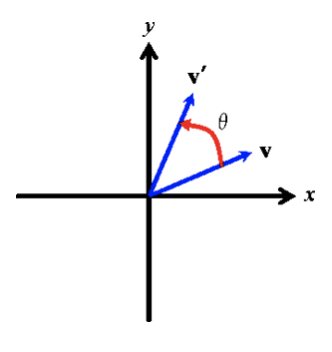
\includegraphics[width=\textwidth]{./images/rotation.png}
    \caption{Rotation}
  \end{minipage}
  \hfill
  \begin{minipage}[b]{0.3\textwidth}
    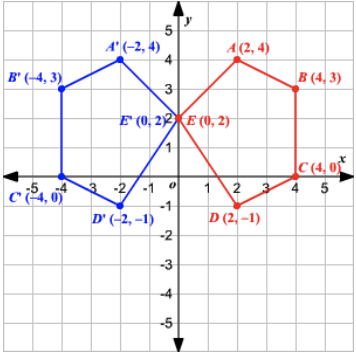
\includegraphics[width=\textwidth]{./images/reflection.png}
    \caption{Reflection}
  \end{minipage}
\end{figure}
\end{frame}



\begin{frame}[t]\vspace{10pt}
\frametitle{Rotation Matrix}
The rotation matrix rotates points by a specified angle, theta: \\~\\
$R(\theta) = \begin{bmatrix}
\cos{\theta} & -\sin{\theta} \\
\sin{\theta} & \cos{\theta} \\
\end{bmatrix}$

Use this matrix by plugging in desired rotation angle, then multiply with vector. \\
\textbf{Note: } Rotation matrices also preserve the length of a vector. \\~\\
\textbf{Example}: Rotation Matrix that rotates vector by $90^{\circ}$ \\~\\
$R(90^{\circ}) = \begin{bmatrix}
0 & -1 \\
1 & 0 \\
\end{bmatrix}$
\end{frame}

\begin{frame}[t]\vspace{10pt}
\frametitle{Rotation Matrix}
The rotation matrix rotates points by a specified angle, theta: \\~\\
$R(\theta) = \begin{bmatrix}
\cos{\theta} & -\sin{\theta} \\
\sin{\theta} & \cos{\theta} \\
\end{bmatrix}$

Use this matrix by plugging in desired rotation angle, then multiply with vector. \\
\textbf{Note: } Rotation matrices also preserve the length of a vector. \\~\\
\textbf{Example}: Rotation Matrix that rotates vector by $90^{\circ}$ \\~\\
$R(90^{\circ}) = \begin{bmatrix}
0 & -1 \\
1 & 0 \\
\end{bmatrix}$
\end{frame}

\begin{frame}[t]\vspace{10pt}
\frametitle{Reflection Matrix}

The reflection matrix reflects vectors across a line (Notice that such matrix also preserves the length of a vector)\\~\\
Notable reflection matrices:

\begin{figure}
  \begin{minipage}{.5\linewidth}
    \centering
    \[\left[\begin{array}{cc}
      1 &  0\\
      0 & -1
    \end{array}\right]\]
    Reflection across $x$-axis
  \end{minipage}%
  \begin{minipage}{.5\linewidth}
    \centering
    \[\left[\begin{array}{cc}
      -1 &  0\\
      0 & 1
    \end{array}\right]\]
    Reflection across $y$-axis
  \end{minipage}
  \begin{minipage}{.5\linewidth}
    \centering
    \[\left[\begin{array}{cc}
      0 & 1\\
      1 & 0
    \end{array}\right]\]
    Reflection across $y=x$
  \end{minipage}
\end{figure}
\end{frame}



\begin{frame}[t]\vspace{10pt}
\frametitle{Matrix Transformations}
All linear transformations can be expressed as a matrix

\begin{figure}[!tbp]
  \centering
  \begin{minipage}[b]{0.45\textwidth}
    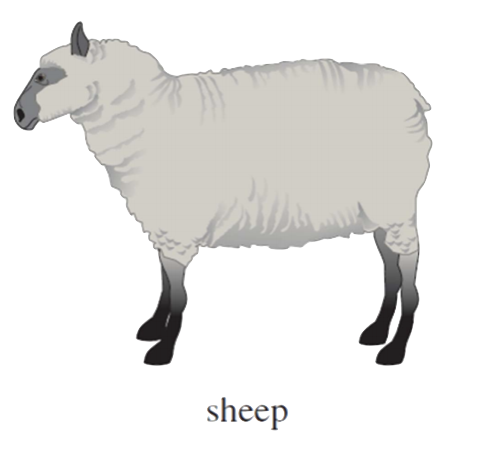
\includegraphics[width=\textwidth]{./images/sheep.png}
  \end{minipage}
  \hfill
  \begin{minipage}[b]{0.45\textwidth}
    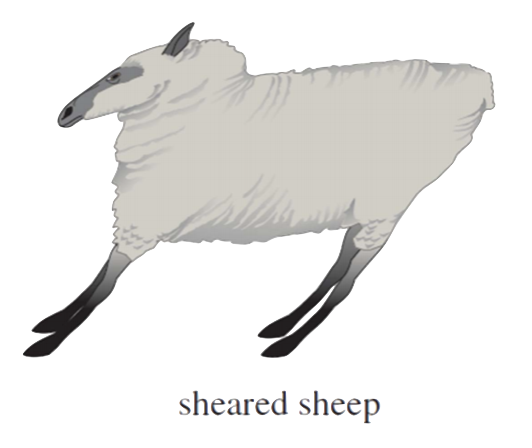
\includegraphics[width=\textwidth]{./images/sheep_shear.png}
  \end{minipage}
\end{figure}
\end{frame}


\begin{frame}[t]\vspace{-10pt}
\frametitle{Example 1}
\only<1>{\makeheader{Question}}
\only<2>{\makeheader{\textcolor{red}{Solution}}}

What is the resulting vector after the following (non-subsequent) transformations are applied 
to the vector 
$\vec{v}= \begin{bmatrix}
2 \\ 3
\end{bmatrix}$
\\~\\

\begin{enumerate}
\setcounter{enumi}{0}
\item Rotate by $45^{\circ}$
\end{enumerate}

\only<1>{\vspace{30pt}}

\only<2>{
\vspace{-10pt}
\[
\begin{bmatrix}
    \cos{45^{\circ}}  &  -\sin{45^{\circ}}      \\
    \sin{45^{\circ}}  &  \cos{45^{\circ}}    
\end{bmatrix}
= 
\begin{bmatrix}
    \frac{\sqrt{2}}{2}  &  -\frac{\sqrt{2}}{2}      \\
    \frac{\sqrt{2}}{2}  &  \frac{\sqrt{2}}{2}      
\end{bmatrix} 
\begin{bmatrix}
    2 \\ 3
\end{bmatrix} 
=
\begin{bmatrix}
 - \frac{\sqrt{2}}{2} \\
 	\frac{5\sqrt{2}}{2}
\end{bmatrix}
\]

}

\begin{enumerate}
\setcounter{enumi}{1}
\item Reflect across $y = x$
\end{enumerate}

\only<2>{
\vspace{-10pt}
\[
\begin{bmatrix}
    0 & 1 \\ 1 & 0
\end{bmatrix} 
\begin{bmatrix}
    2 \\ 3
\end{bmatrix} 
=
\begin{bmatrix}
 3\\2
\end{bmatrix}
\]
}
\end{frame}


\begin{frame}[t]\vspace{10pt}
\frametitle{Determinants}
Determinant of a $2 x 2$ matrix: \\
\[ 
det \, (
\begin{bmatrix} a & b \\ c & d \end{bmatrix}
)
= ad - bc
\]

Also, an upper triangular matrix’s determinant is the product of the diagonal: \\
\[ 
det \, (
\begin{bmatrix} 
a & * & * & \cdots \\
0 & b & * & \cdots \\
0 & 0 & c & \cdots \\
\vdots & \vdots & \vdots & \ddots \\
 \end{bmatrix}
)
= abc \cdots
\]
\end{frame}



\begin{frame}[t]\vspace{10pt}
\frametitle{Gaussian Elimination}
\textbf{Ultimate goal: } Upper triangular form (\textbf{i.e} numbers below the diagonal are all 0) \\~\\
\textbf{Reminder of Motivation:} Can work starting from the bottom row up in order to quickly calculate (from a computer’s perspective) each variable’s value. \\
For example, the last row has one variable and one value. 
\end{frame}


\begin{frame}[t]\vspace{10pt}
\frametitle{Gaussian Elimination}
\textbf{IDEA: } Augmented matrix represents a system of equations where each row is an equation. \\
What are you allowed to do with equations to solve them?

\begin{enumerate}
\item \textbf{Row exchange} (same equations,  different order)
\item \textbf{Scaling} (multiplying an equation by  a scalar)
\item \textbf{Replace a row with the a linear combination of itself and another row} (intuitively, must include itself because otherwise there is “loss of information”, like a deletion of one of the original rows)
\end{enumerate}

\textbf{GOAL:} \\ Original Matrix $\rightarrow$ Row Echelon Form $\rightarrow $ Reduced Row Echelon Form
\end{frame}


\begin{frame}[t]\vspace{-10pt}
\frametitle{Gaussian Elimination Example}
\only<1>{\makeheader{Problem}}
\only<2>{\makeheader{\textcolor{red}{Solution}}}
Use Gaussian Elimination to reduce the following system of equations:\\~\\

% https://tex.stackexchange.com/questions/35174/best-way-to-create-an-system-of-equations-environment
\only<1> {
\[
  \spalignsys{
    x_1 +  x_2 + x_3 = 8;
    2x_1 - 4x_2 +  3x_3 =  9 ;
    -x_1 + 5x_2 - 2x_3 = 0
  }
\]
}
\only<2>{
$
  \begin{bmatrix}[ccc|c]
  1 & 1 & 1 & 8\\
  2 & -4 & 3 & 9\\
  -1 & 5 & -2 & 0
  \end{bmatrix}
  \xrightarrow[]{2R_1 - R_2 \rightarrow R_2 }
  \begin{bmatrix}[ccc|c]
  1 & 1 & 1 & 8\\
  0 & 6 & -1 & 7\\
  -1 & 5 & -2 & 0
  \end{bmatrix}
  \xrightarrow[]{R_1 + R_3 \rightarrow R_3 }
$

\vspace{10pt}

$
  \begin{bmatrix}[ccc|c]
   1 & 1 & 1 & 8\\
   0 & 6 & -1 & 7\\
   0 & 6 & -1 & 8
  \end{bmatrix}
  \xrightarrow[]{R_2 - R_3 \rightarrow R_3  }
  \begin{bmatrix}[ccc|c]
  1 & 1 & 1 & 8\\
   0 & 6 & -1 & 7\\
  0 & 0 & 0 & -1
  \end{bmatrix} 
$

The last row implies 0 of three variables add up to -1. Therefore, there exists no solution.
}
\end{frame}


\begin{frame}[t]\vspace{10pt}
\frametitle{Possible Outcomes from Gaussian Elimination}

\hspace*{-2pt}\makebox[\linewidth][c]{
\begin{tiny}
\begin{tabular}{p{2.5cm} | p{2.5cm} | p{2.5cm} | p{2.5cm}}

\textbf{Possible Results} & Row Picture & Column Picture & Properties of Matrix A\\
\hline \hline
\textbf{Unique solution} & Equations intersect at exactly one point & \textbf{b} can be uniquely represented by the linear combination of the columns of  \textbf{A} &  \textbf{A} is invertible \\
\hline
\textbf{Infinite solutions} & Equations intersect along an infinite space (eg. the intersection is a line or a plane) & There are multiple ways of representing \textbf{b} in terms of the linear combination of the columns of \textbf{A} & \textbf{A} has linearly dependent columns \\
\hline
\textbf{No solutions} & Equations do not intersect & \textbf{b} is not in the span of the columns of \textbf{A}; \textbf{b} is not in the column space of \textbf{A} & Column space of \textbf{A} does not contain (span) the vector \textbf{b}
\end{tabular}
\end{tiny}
}


\end{frame}

\section*{Linear (In)dependence \& Invertibility}

\begin{frame}
\frametitle{Linear Combination}
Core: Addition and Scaling \\
In context of vectors $v_1, v_2, \ldots, v_n$:\\
\[a_1 v_1 + a_2 v_2 + \cdots + a_n v_n\] \\
where $a_1, a_2, \ldots, a_n$ are scalars
\end{frame}

\begin{frame}
\frametitle{Taking a Step Back}
Hopefully by now you have been able to recognize that the core of all linear algebra is linear combinations. \\
Think back to how one of the rules of row operations allows to a linear combination of rows as long as the original row being replaced is included!
\end{frame}

\begin{frame}
\frametitle{Column Space}
Let $v_1, v_2, \dots, v_n$ be the columns of matrix $V$. The linear combination of the vectors is the \textbf{Column Space} of $V$. \\
This is also known as the \textbf{Range} of $V$, because when a matrix multiplies a vector or another matrix (which is just multiple vectors!), the result is a linear combination of all the columns. Hence, the linear combination of the columns is like the reach, or \textbf{Range} of the matrix.
\end{frame}

\begin{frame}
\frametitle{Linear Dependence: Two Definitions}
\begin{enumerate}[(i)]
\item A set of vectors $\{ v_1, \ldots, v_n \}$ is linearly dependent if there exist scalars $a_1, \ldots, a_n$ such that $a_1 v_1 + a_2 v_2 + \cdots + a_n v_n = 0$ and not all $a_i$'s are $0$.
\item A set of vectors is linearly dependent if one of the vectors could be written as a linear combination of the rest of the vectors. $v_i = \sum_{j \neq i} a_j v_j$.
\end{enumerate}
\end{frame}

\begin{frame}
\frametitle{Linear Independence}
Strictly speaking, a matrix is linearly independent if it is \textbf{not} linearly dependent.\\
In other words, for a set of linearly independent vectors, $a_1 v_1 + a_2 v_2 + \cdots + a_n v_n = 0$ implies that all $a_1 = 0, a_2 = 0, \cdots , a_n = 0$ (useful when doing proofs).
\end{frame}

\begin{frame}
\frametitle{Linear (In)dependence}
Conceptually, if you have $2$ equations and $3$ unknowns, you cannot solve it. Imagine if you have $3$ equations but one equation was actually a linear combination of the first two. You still have the same ``information'' of $2$ equations as your ``basis''. Many important implications.
\end{frame}

\begin{frame}
\frametitle{Span}
The \textbf{span} of a set of vectors $\{v_1, \ldots, v_n\}$ is the set of all linear combinations of $\{v_1, \ldots, v_n\}$.\\
In other words, if one vectors $v_i$ in a set of $n$ vectors lied in the span of the other vectors, then that set is considered linearly dependent.
\end{frame}

\begin{frame}
\frametitle{Rank}
The \textbf{rank} of a matrix $A$ is the dimension of the column space of $A$. \\
This is the same as the number of linearly independent column vectors. \\
This is also the same as the number of linearly independent row vectors.
\end{frame}

\begin{frame}
\frametitle{Relating it Back To Linear (In)dependence}
Colloquially, a matrix $A$ can be said to \textbf{span} $n$ dimensions. \\
This means that matrix $A$ has $n$ linearly independent rows and $n$ linearly independent columns. \\
This also means that matrix $A$ is of \textbf{rank} $n$.
\end{frame}

\begin{frame}
\frametitle{Span \& Rank \& (In)dependence}
To figure out the \textbf{span} of a set of vectors, think of them as the column vectors of a matrix and Gaussian eliminate that matrix to RREF. \\
The number of non-zero rows is the \textbf{dimension} the vectors span. \\
If those vectors were actually the columns of a matrix, the dimension is also the \textbf{rank} of that matrix. \\
If the dimension is the same as the total number of vectors, then those vectors are \textbf{independent}.
\end{frame}

\begin{frame}
\frametitle{\only<2>{SOL: }Example of figuring out Span \& Rank}
\[
\begin{bmatrix}
1 & 2 & 1 & -4\\
0 & -1 & 1 & -2\\
1 & 4 & 1 & 2\\
\end{bmatrix}
\uncover<2>{
\xrightarrow{R_3 - R_1 \rightarrow R_3}
\begin{bmatrix}
1 & 2 & 1 & -4\\
0 & -1 & 1 & -2\\
0 & 2 & 0 & 6\\
\end{bmatrix}
\]
\[
\xrightarrow{R_2 \leftrightarrow \frac{1}{2} R_3}
\begin{bmatrix}
1 & 2 & 1 & -4\\
0 & 1 & 0 & 3\\
0 & -1 & 1 & -2\\
\end{bmatrix}
\xrightarrow{R_2 + R_3 \rightarrow R_3}
\begin{bmatrix}
1 & 2 & 1 & -4\\
0 & 1 & 0 & 3\\
0 & 0 & 1 & 1\\
\end{bmatrix}
\]
\begin{center}
There are 3 linearly independent rows!
\end{center}}
\end{frame}

\begin{frame}
\frametitle{Inverses}
A matrix $A$ is \textbf{invertible} if $A$ is a square matrix of \textbf{rank} $n$ where $n$ is the number of rows and columns. (This means linearly independent rows/cols.) \\
If a matrix $A$ is invertible, then there exists a matrix $B$ such that $AB=BA=I$, where $I$ is the identity matrix. \\
Normally notated as: $A^{-1}$
\end{frame}

\begin{frame}
\frametitle{Inverse Matrix Properties}
\[AA^{-1} = A^{-1}A = I\]
\[(A^{-1})^{-1} = A\]
\[(kA)^{-1} = \frac{1}{k} A^{-1}\]
\[(AB)^{-1} = B^{-1} A^{-1}\]
\end{frame}

\begin{frame}
\frametitle{Finding the inverse}
Construct an $n$ x $2n$ augmented matrix: \\
\[ [A \mid I] \]
Row reduce until the left becomes the identity; the right is the inverse \\
\[ [A \mid I] \sim \ldots \sim [I \mid A^{-1}] \]
\end{frame}

\begin{frame}
\frametitle{Cheat sheet: $2$x$2$ Inverse}
\[
A^{-1} =
\begin{bmatrix}
a & b\\
c & d\\
\end{bmatrix}^{-1}
= \frac{1}{ad-bc}
\begin{bmatrix}
d & -b\\
-c & a\\
\end{bmatrix}
\]
\end{frame}

\begin{frame}
\frametitle{\only<2>{SOL: }Inverse Example}
\[
\begin{bmatrix}[ccc|ccc]
1 & 3 & 3 & 1 & 0 & 0\\
1 & 4 & 3 & 0 & 1 & 0\\
1 & 3 & 4 & 0 & 0 & 1\\
\end{bmatrix}
\uncover<2>{
\xrightarrow{R_2 - R_1 \rightarrow R_2}
\begin{bmatrix}[ccc|ccc]
1 & 3 & 3 & 1 & 0 & 0\\
0 & 1 & 0 & -1 & 1 & 0\\
1 & 3 & 4 & 0 & 0 & 1\\
\end{bmatrix}
\xrightarrow{R_3 - R_1 \rightarrow R_3}
\]
\[
\begin{bmatrix}[ccc|ccc]
1 & 3 & 3 & 1 & 0 & 0\\
0 & 1 & 0 & -1 & 1 & 0\\
0 & 0 & 1 & -1 & 0 & 1\\
\end{bmatrix}
\xrightarrow{R_1 - 3R_2 \rightarrow R_1}
\begin{bmatrix}[ccc|ccc]
1 & 0 & 3 & 4 & -3 & 0\\
0 & 1 & 0 & -1 & 1 & 0\\
0 & 0 & 1 & -1 & 0 & 1\\
\end{bmatrix}
\]
\[
\xrightarrow{R_1 - 3R_3 \rightarrow R_1}
\begin{bmatrix}[ccc|ccc]
1 & 0 & 0 & 7 & -3 & -3\\
0 & 1 & 0 & -1 & 1 & 0\\
0 & 0 & 1 & -1 & 0 & 1\\
\end{bmatrix}
\]
}
\end{frame}

\section*{Break!}

\section*{Nullspace/Vector Space/Basis/Subspace}

\begin{frame}
    \frametitle{Vector Spaces}
    \textbf{A set of elements closed under vector addition and scalar multiplication} \\
    Properties of a vector space $V$: \\
    \begin{enumerate}
        \item If $u$ and $v$ are vectors in $V$, then $u+v$ must be in $V$ \\
        \item If $u$ is a vector in $V$ and $k$ is a real number, then $ku$ must be in $V$ \\
    \end{enumerate}
    * Any linear combination of vectors in $V$ is still in $V$ (the span of a vector space is itself).
\end{frame}

\begin{frame}
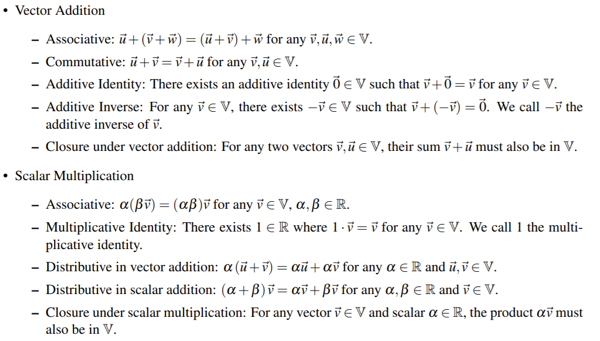
\includegraphics[width=\textwidth]{./images/vector_space_properties.png}
\end{frame}

\begin{frame}
    \frametitle{Practice: Vector Space or Not?}
    \begin{itemize}
        \item $2$D plane, (two vectors spanning $\mathbb{R}^2$) \only<2>{\textcolor{red}{(Yes)}}
        \item $5$D space, (five vectors spanning $\mathbb{R}^5$) \only<2>{\textcolor{red}{(Yes)}}
        \item $n$-D space, ($n$ vectors spanning $\mathbb{R}^n$) \only<2>{\textcolor{red}{(Yes)}}
        \item Line in $\mathbb{R}^2$ \only<2>{\textcolor{red}{(It depends)}}
        \begin{itemize}
            \item Intersecting origin \only<2>{\textcolor{red}{(Yes)}}
            \item Not intersecting origin \only<2>{\textcolor{red}{(No)}}
        \end{itemize}
    \item First and third quadrant of $\mathbb{R}^2$ \only<2>{\textcolor{red}{(No)}}
    \item Plane in $\mathbb{R}^3$ intersecting origin \only<2>{\textcolor{red}{(Yes)}}
    \item $\{ 0 \}$ (Just the zero vector) \only<2>{\textcolor{red}{(Yes)}}
    \item $\{ v \in \mathbb{R}^n \mid v \neq 0 \}$ \only<2>{\textcolor{red}{(No)}}
    \end{itemize}
\end{frame}

\begin{frame}
    \frametitle{Subspaces}
    \textbf{A subspace is a subset of a vector space that is itself a vector space} \\
    Suppose we have a vector space $V$. A subset $S$ of $V$ is only a subspace if the following three properties are met: \\
    \begin{enumerate}
        \item The zero vector of $V$ is in $S$
        \item $S$ is closed under vector addition. $u + v \in S$
        \item $S$ is closed under multiplication by scalars. $cu \in S$
    \end{enumerate}
    (Same rules as before!)
\end{frame}

\begin{frame}
    \frametitle{Bases}
    A \textbf{basis} of a vector space is a \textbf{linearly independent} set of vectors that \textbf{span} the vector space.
    \begin{enumerate}
        \item All vectors in the set are \textbf{linearly independent}
        \item All vectors in the vector space can be represented as a linear combination of the basis vectors (\textbf{span}).
    \end{enumerate}
\end{frame}

\begin{frame}
    \frametitle{Bases}
    A basis does not necessarily have to span $\mathbb{R}^n$ - it can span any vector space.
    \begin{itemize}
        \item A basis is a \textbf{minimum set of vectors} required to completely span a vector space.
        \begin{itemize}
            \item e.g. Any basis of $\mathbb{R}^n$ contains \textbf{exactly} $n$ vectors. In fact, an $m$-dimensional vector space must have $m$ vectors in its basis.
        \end{itemize}
        \item Bases are NOT unique! Why? How many are there?
    \end{itemize}
\end{frame}

\begin{frame}
    \frametitle{Nullspace}
    The null space of a matrix (transformation) is the set of all solutions to the homogeneous equation $Ax=0$. It is a subspace of $\mathbb{R}^n$. \\
    Finding a null space:
    \begin{enumerate}
        \item Reduce to reduced row-echelon form, identify free variables
        \item Write out system of equations, represent solutions in matrix form
        \item Write out linear combination of vectors with free variables as coefficients
        \item The vectors are the basis of the null space
    \end{enumerate}
\end{frame}

\begin{frame}[t]\vspace{0pt}
    \frametitle{Example of Solving Nullspace}
    \[
    \begin{bmatrix}
    -3 & 6 & -1 & 1 & -7\\
    1 & -2 & 2 & 3 & -1\\
    2 & -4 & 5 & 8 & 2\\
    \end{bmatrix}
    \xrightarrow{\text{Row Reduce}}
    \begin{bmatrix}
    1 & -2 & 0 & -1 & 0\\
    0 & 0 & 1 & 2 & 0\\
    0 & 0 & 0 & 0 & 1\\
    \end{bmatrix}
    \]
    Goal is finding all $x$ where $Ax=0$ \\
    \only<1>{
    A matrix will have the \textbf{same nullspace} as its row reduced form. \\
    This is because row reducing is the same as manipulating equations; the solution for the row reduced form is the same as the solution for the original matrix.
    }
    \only<2>{
    \begin{small}
    \begin{minipage}{.5\linewidth}
        Let $x = \begin{bmatrix} x_1 & x_2 & x_3 & x_4 & x_5 \end{bmatrix}^T$ \\
        Rewrite in system of equations: \\
        $x_1 - 2x_2 - x_4 = 0 \implies x_1 = 2x_2 + x_4$ \\
        $x_3 + 2x_4 = 0 \implies x_3 = -2x_4$ \\
        $x_5 = 0$
    \end{minipage}%
    \begin{minipage}{.52\linewidth}
        Let $u=x_2$, $v=x_4$. Then: \\
        $\begin{bmatrix} x_1 \\ x_2 \\ x_3 \\ x_4 \\ x_5 \end{bmatrix}
        = \begin{bmatrix} 2u + v \\ u \\ -2v \\ v \\ 0 \end{bmatrix}
        = \begin{bmatrix} 2 \\ 1 \\ 0 \\ 0 \\ 0 \end{bmatrix} u
        + \begin{bmatrix} 1 \\ 0 \\ -2 \\ 1 \\ 0 \end{bmatrix} v$
    \end{minipage}
    So the null space is the span of $\begin{bmatrix} 2 & 1 & 0 & 0 & 0 \end{bmatrix}^T$ and $\begin{bmatrix} 1 & 0 & -2 & 1 & 0 \end{bmatrix}^T$ because multiplying $A$ by any linear combination of those two vectors equals $0$.
    \end{small}
    }
\end{frame}

\begin{frame}
    \frametitle{Addition to Invertibility}
    If a matrix has a nontrivial nullspace (does not only contain the $0$ vector), then it is not invertible. (Same as saying a matrix is invertible iff its nullspace is trivial i.e. only contains the $0$ vector.) \\
    Intuitive explanation: If $Av=0$ where $v \neq 0$, then the nullspace at least contains the span of $v$. There are then infinite solutions to $Au=0$. So $A^{-1}$ does not exist.
\end{frame}

\end{document}
